\documentclass[a4paper]{scrreprt}

% Uncomment to optimize for double-sided printing.
% \KOMAoptions{twoside}

% Set binding correction manually, if known.
% \KOMAoptions{BCOR=2cm}

% Localization options
\usepackage[english]{babel}
\usepackage[T1]{fontenc}
\usepackage[utf8]{inputenc}

% Quotations
\usepackage{dirtytalk}

% Floats
\usepackage{float}

% Enhanced verbatim sections. We're mainly interested in
% \verbatiminput though.
\usepackage{verbatim}

% Automatically remove leading whitespace in lstlisting
\usepackage{lstautogobble}

% PDF-compatible landscape mode.
% Makes PDF viewers show the page rotated by 90°.
\usepackage{pdflscape}

% Advanced tables
\usepackage{array}
\usepackage{tabularx}
\usepackage{longtable}

% Fancy tablerules
\usepackage{booktabs}

% Graphics
\usepackage{graphicx}

% Current time
\usepackage[useregional=numeric]{datetime2}

% Float barriers.
% Automatically add a FloatBarrier to each \section
\usepackage[section]{placeins}

% Custom header and footer
\usepackage{fancyhdr}

\usepackage{geometry}
\usepackage{layout}

% Math tools
\usepackage{mathtools}
% Math symbols
\usepackage{amsmath,amsfonts,amssymb}
\usepackage{amsthm}
% General symbols
\usepackage{stmaryrd}

% Utilities for quotations
\usepackage{csquotes}

% Bibliography
\usepackage[
  style=alphabetic,
  backend=biber, % Default backend, just listed for completness
  sorting=ynt % Sort by year, name, title
]{biblatex}
\addbibresource{references.bib}

\DeclarePairedDelimiter\abs{\lvert}{\rvert}
\DeclarePairedDelimiter\floor{\lfloor}{\rfloor}

% Bullet point
\newcommand{\tabitem}{~~\llap{\textbullet}~~}

\pagestyle{plain}
% \fancyhf{}
% \lhead{}
% \lfoot{}
% \rfoot{}
% 
% Source code & highlighting
\usepackage{listings}

% SI units
\usepackage[binary-units=true]{siunitx}
\DeclareSIUnit\cycles{cycles}

\newcommand{\lecture}{41109 - Privacy and Data Security}
\newcommand{\series}{03}
% Convenience commands
\newcommand{\mailsubject}{\lecture - Series \series}
\newcommand{\maillink}[1]{\href{mailto:#1?subject=\mailsubject}
                               {#1}}

% Should use this command wherever the print date is mentioned.
\newcommand{\printdate}{\today}

\subject{\lecture}
\title{Series \series}

\author{Michael Senn \maillink{michael.senn@students.unibe.ch} --- 16-126-880}

\date{\printdate}

% Needs to be the last command in the preamble, for one reason or
% another. 
\usepackage{hyperref}

\begin{document}
\maketitle


\setcounter{chapter}{\numexpr \series - 1 \relax}

\chapter{Series \series}

\section{Physical security versus logical security}

Observe first that, for logical security, the outer layers derive their
security from the inner layers. As an example full access to the hardware
grants an attacker full access to all the layers surrounding it, up to the
application in the outermost layer.

In the case of physical security, each layer can be thought of as a separate
`wall' which has to be bypassed in sequence. Being able to bypass one specific
layer of physical security --- e.g. the door to the server room --- does not
help with bypassing either the perimeter fence or the lock on the server rack.

Combining these two models into a coherent `combined and integrated model of
physical and logical security' is a bit peculiar. One could think of a
triangle. At its top sits the hardware, the most `sensitive' component common
to both models. Along the left side of the triangle are, in sequence, the
layers of physical security. Along the right side of the triangle are, in
sequence, the layers of logical security.

An attacker then has the goal of getting as far up the triangle as possible.
He has the choice of either ascending the left side, breaking through layers of
physical security, or ascending the right side, breaking through layers of
logical security. Once he reached the top he has full access to the whole
system.

However this model is lacking in that it might focus too much on the paths an
attacker can take, rather than on the goals of security. Consider that the one
component one usually wants to protect is the application and its data which,
in this model, sits at the very edge.

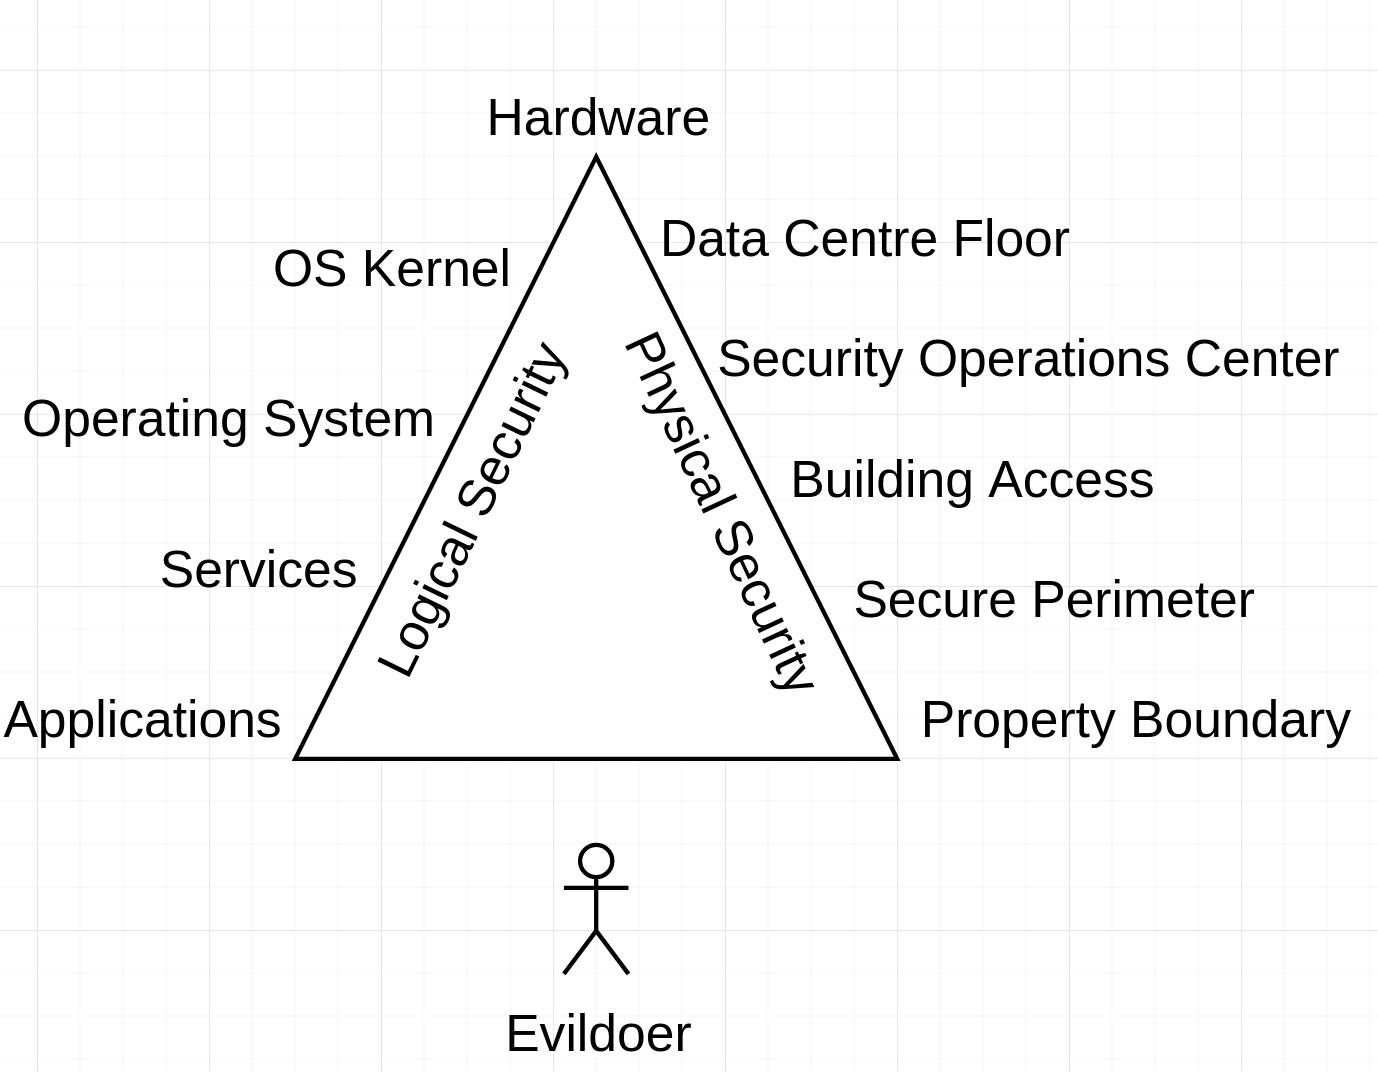
\includegraphics[width=\textwidth]{combined_security_model}

\section{How to hide a logical bomb}

\subsection{Importance of $H$ being a one-way function}

$H$ being a one-way function is essential as it ensures that knowledge of the
`trigger' --- based on the key $K$ and the function $H$ --- does not provide
any information about the key $K$. If $H$ was easily invertible, then an
attacker could calculate the key using publically available information.  As an
example consider the proposed ``blind search'' scheme, where the trigger $O$ is
defined as $O = H(N \oplus K)$ for a nonce $N$. The key would then easily
follow as $K = H^{-1}(O) \oplus N$. Similar results are possible for all
other proposed schemes, if $H$ were not a one-way function.

\subsection{Guarding against malicious code}

In order for an execution environment to guard itself against environmental
keys as described in the paper, could attempt to mask as much environmental
information as possible. As an example consider that, instead of exposing
actual DNS information, it would expose randomized (but deterministic within
the context of each participant) information to each participant. This way,
environmental information could not reliably be used to determine an encryption
key.

Clearly such defense mechanisms will often interfere with regular operation of
the execution environment though, as they also affect all benevolent programs
relying on the masked environmental information.

As such, different approaches, which allow for a more generic defense against
malicious code, seem more suitable to use. The most popular one, used
extensively in browsers, is to provide a sandboxed environment for potentially
malicious code to run in. The code can then only access resources exposed to
the sandbox, and interface with the outside world --- if at all --- through a
tightly controlled interface. As mentioned such an approach does have the
advantage of being applicable to all kinds of potentially malicious code,
rather than specifically code using environmental keys.

\printbibliography

\end{document}
